% Template - https://sanskrit.uohyd.ac.in/18WSC/Style_files/CS_and_DH.tex
\providecommand{\tightlist}{%
  \setlength{\itemsep}{0pt}\setlength{\parskip}{0pt}}

\documentclass[11pt]{article}
\usepackage{scl}
\usepackage{times}
\usepackage{url}
\usepackage{latexsym}
\usepackage{lineno}

\usepackage{fontspec, xunicode, xltxtra}
\newfontfamily\skt[Script=Devanagari]{Sanskrit 2003}
\setmonofont{Sanskrit 2003}


\title{A browser-side-dynamic website framework for annotated Indic texts}

\author{
  Vishvas Vasuki \\
  Dyugaṅgā, Beṅgaḷūru \\
  {\tt https://sanskrit.github.io/groups/dyuganga/}
\\}

\date{}

\begin{document}
\maketitle
%\linenumbers
\begin{abstract}
Perusing Indic classics on the web is an increasingly popular activity. However, serving and maintaining feature-rich websites involves significant costs, knowledge and effort. We present an easy to use website framework to mitigate these drawbacks. Besides being simple and low-cost, the proposed solution is rich in features particularly useful for presenting Indic language classics - including easy transliteration, navigation aids, annotation support, dynamic content inclusion and more.
\end{abstract}

\section{Motivation}
The advent of internet, personal computers and mobile devices have radically changed the way we consume literature. We can now carry an entire library in our pockets. Besides access to simple text, digital readers are able to utilize features such as text-to-speech, embedded multimedia, easy navigation and dictionary lookup. 

On the production end - publishing on the web is far simpler and cheaper than publishing paper books. Yet, doing it well (i.e. with the dynamic features digital readers expect) still involves significant costs, knowledge and effort. Furthermore, for highly structured texts - like originals with series of commentaries and translations - content management becomes non-trivial.

We present a framework to publish annotated Indic language texts, providing the following features:

\begin{itemize}
\tightlist
\item
  \textbf{Content management}

  \begin{itemize}
  \tightlist
  \item
    ``Suggest edits'' links, which work when the content is stored in an online Github-like repository.
  \item
    Basic ability to include contents from another page using the same
    theme within another.
  \item
    Inline annotation
  \item
    It's easy to copy or export the underlying content.
  \item
    Version control is available when backed by a GitHub-type online repository.
  \item
    Very low operating costs \footnote{Zero cost if services like GitHub Pages are used.} - only a simple web page server is needed - no database server or ability to run custom code on server is required.
  \end{itemize}
\item
  \textbf{Navigation}

  \begin{itemize}
  \tightlist
  \item
    Collapsible ``accordion'' sidebar with automated directory listing.
  \item
    Collapsible ``accordion'' table-of-contents for each page.
  \item
    ``Next and Previous'' page navigation buttons.
  \end{itemize}
\item
  \textbf{Search}

  \begin{itemize}
  \tightlist
  \item
    JSON based title/ url search
  \item
    Search engine optimization markup and indices - which you would use
    with various search engines.
  \end{itemize}
\item
  \textbf{Reading}

  \begin{itemize}
  \tightlist
  \item
    A layout which automatically adjusts to the user's screen size.
  \item
    Embedding audio and video items. Ability to sequentially play audio
    tracks within a page.
  \item
    Transliteration dropdown: scripts ranging from devanāgarī to
    grantha, brāhmī to ISO-15919.
  \item
    Special formatting consideration for fonts which need to be
    displayed bigger (eg: Devanagari for sanskrit.)
  \item
    Text to speech interface (under development).
  \item
    Disqus for comments.
  \item
    Collapsible detail sections.
  \end{itemize}
\end{itemize}


This framework has been used in several websites, such as \cite{vishvAsa_kalpAntaram}, \cite{vishvAsa_kannada} and \cite{vishvAsa_bhAShAntaram}.


\begin{figure}[h]
\caption{Screenshot of a website}
\centering
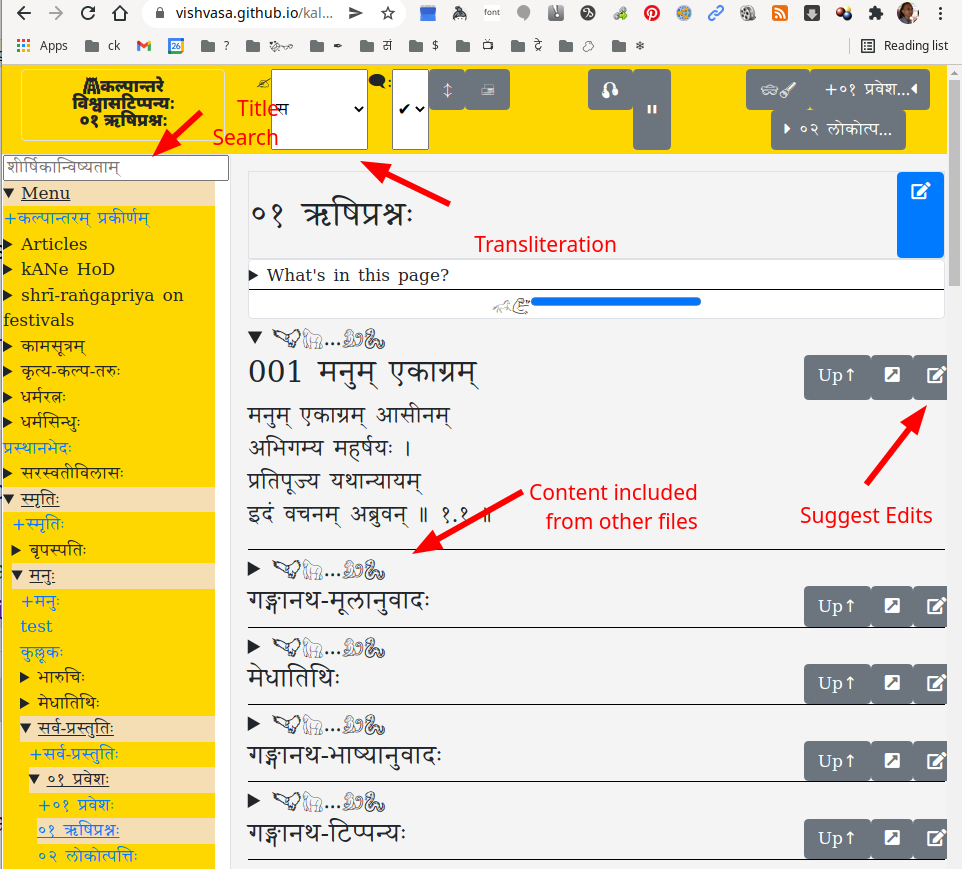
\includegraphics[width=1.0\textwidth]{images/kalpAntaram-screenshot}
\end{figure}


\section{Content format}
Content is stored in the form of plain text files with Markdown content \cite{commonmark} and YAML or TOML metadata headers \cite{toml}. 

\subsection{Markdown}
The advantage of Markdown is that it is very simple and intuitive - while having most basic features (such as sectioning, bold text, italics, lists, footnotes, images). One can edit markdown with just a plain text editor, without the need of special editing software as in the case of TEI \footnote{TEI is a popular XML-based format for storing structured Sanskrit texts. With XML, as in the case of HTML, the tags begin to eclipse the content - making plain text editing cumbersome.}. 

Markdown format is very popular, and is supported by several parsers in popular programming languages, with HTML being most common target language. This makes the content highly portable accross display software (including static website generators).

An example file is as follows:

\begin{verbatim}
+++
english_title = "001 nārada briefs vālmīki about rāma"
title = "००१ सङ्क्षेपरामायणम्"
unicode_script = "devanagari"

+++
## नारदाय प्रश्नः

तपस्स्वाध्यायनिरतं तपस्वी वाग्विदां वरम् ।  
नारदं परिपप्रच्छ वाल्मीकिर्मुनिपुङ्गवम् ॥1.1.1॥

कोन्वस्मिन्साम्प्रतं लोके गुणवान्कश्च वीर्यवान् ।  
धर्मज्ञश्च कृतज्ञश्च सत्यवाक्यो दृढव्रतः॥1.1.2॥

चारित्रेण च को युक्तस्सर्वभूतेषु को हितः ।  
विद्वान्कः कस्समर्थश्च कश्चैकप्रियदर्शनः ॥1.1.3॥

...
\end{verbatim}

\subsection{Extensions to Markdown}
Basic markdown can be enhanced with HTML code as needed - but we recommend being conservative about it as adding too much HTML almost never necessary, and HTML code can begin to obscure content and reduce plain-text readability. We have found the details tag to be particularly useful to produce collapsible boxes; for example:

\begin{verbatim}
<details><summary>मूलम्</summary>

क्व सूर्य-प्रभवो वंशः  
क्व चाल्पविषया मतिः ।  
तितीर्षुर् दुस्तरम् मोहाद्  
उडुपेनास्मि सागरम् ॥ २ ॥    
</details>
\end{verbatim}

Occassionally, we embedding find page-specific scripts useful as well, using the regular \verb'<script>' tag (for example to open a random verse or stotra upon visiting a certain URL). <u> is also used to underline text.

\subsubsection{Content inclusion}
In addition to this, our framework fetches and fills in markdown/ text/ HTML content from other URL-s with tags such as the following:


\begin{verbatim}
<div class="js_include" newlevelforh1="4" title="Oldenberg" url="/khAdira/1/02.md"></div>
\end{verbatim} 

We've found such content inclusion to be very useful in managing structured data. 

\begin{itemize}
\tightlist

\item
For example, a particular verse may be associated with 10 commentaries - storing them separately - say in numbered files - replicates the advantages of using a database with the simplicity and convenience of a plain file system. One can edit some commentary without being botherd by the clutter of unrelated content. 

\item
Furthermore, the exact same content (example the r̥k "tat savitur …" with annotation) may be included in multiple texts (example - r̥gvēda, yajurvēda, upākarma ritual procedure …). We're able to avoid having to copy / paste and maintain identical content in multiple locations by efficiently using include directives. 
\end{itemize}

\subsubsection{Embedding data and media}
We can embed tables from - say TSV or TOML files - as spreadsheets using the directive shown below:

\begin{verbatim}
<div class="spreadsheet" src="../sutras.toml" fullHeightWithRowsPerScreen=8> </div>  
\end{verbatim}

Similarly, for embedding multimedia:
\begin{verbatim}
<div class="audeoEmbed"  src="http://www.xyz.com/raghuvaMsha1.mp3"  
caption="Recitation by Kuṭumbaśāstrī"></div>
<div class="videoEmbed"  src="https://www.youtube.com/watch?v=TDNkBFbp9Pk"  
caption="Abhinaya by Padmā"></div>
\end{verbatim}

For figures with caption:
\begin{verbatim}

  
\end{verbatim}

\subsubsection{Inline comments}
A favorite reading practice is to insert one's comments in the middle of some text. With our framework, this can be done as shown below:

\begin{verbatim}
सेना परिच्छदस् तस्य,  
+++(यतः -)+++ द्वयम् एवार्थ-साधनम् ।  
शास्त्रेष्व् अकुण्ठिता बुद्धिर्,  
मौर्वी धनुषि चातता ॥ १९ ॥   
\end{verbatim}

This can be made to yield:


\begin{figure}[h]
\caption{Inline comment display example}
\centering
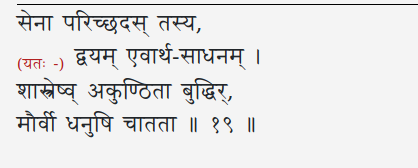
\includegraphics[width=1.0\textwidth]{images/inline-comment-example}
\end{figure}


\subsection{File metadata}
Metadata is stored in TOML or YAML format at the top of the file, as shown in an example earlier. The most important metadata for a given file is it's title. That apart, specifying the script used in the content is important for transliteration and display.

\subsection{Mechanical content management}
Content files are often hand crafted. Others are the generated mechanically from pre-existing content. For example: 

\begin{itemize}
\tightlist
\item
  It may be desirable to split a large content file with multiple sections into multiple different files for ease of navigation and speed. Or one might want to join multiple files into a single file.
\item
  One may want to generate markdown files from pages scraped off some preexisting website.
\item
  One may want to pre-include content within the include directives (mentioned earlier) so as to facilitate proper indexing by search engine crawlers.
\item
  One may want to transliterate content, or add a few commentaries for each verse.
\end{itemize}

For such cases, we have developed an open source python library \cite{doc_curation}, which inturn uses a python transliteration library as needed  \cite{indic_transliteration_py}.

\section{Generating HTML pages}
The content is ultimately presented to the user via a web browser. Hence, HTML pages are generated from content markdown files efficiently. This process can be automated with simple "Continuous Integration" scripts on hosts such as GitHub \cite{vishvAsa_kalpAntaram_src}. For the most part, we use Hugo - a popular static site generation framework \cite{hugo} together with UI templates we've designed as part of our Hugo ``theme" \cite{sandoc_hugo}. \footnote{We initially used \cite{sandoc_jekyll} Jekyll \cite{jekyll}, which is orders of magnitude slower.}

For faster builds, enable some markdown files to be served without parsing them into HTML \footnote{This is accomplished by keeping them within the static folder in case of Hugo.}. They are parsed into HTML as needed on the reader's browser.

\section{Browser side dynamism}
For the convenience of readers, it is essential that the website be interactive. Rather than rely on running custom code on the HTTP server (and incur significant costs and complexity), we rely on the reader's browser. Whereas some of this browser-side dynamism can be accomplished simply via HTML directives (as in the case of details tag or CSS styles), some interactiveness is accomplished via Javascript code (as in the case of navigation, search, content inclusion and transliteration). This code has been incorporated into our Hugo theme \cite{sandoc_hugo}, and is embedded into each webpage generated by the static site generator. An advantage on relying on browser side scripting is that the code is rendered independendent of any particular static website generation software (which oft use custom template languages). 

One disadvantage of relying on Javascript to include or modify content is that it may thwart proper indexing of the generated content by search engine web crawlers. This is potentially caused by rendering delays \footnote{Experience suggests that the Google web crawler, for example, does not wait longer than 5s for the page to be rendered - if it waits at all.}. This problem can be mitigated by mechanically "pre-including" a snapshot of the content to be included at the time the HTML pages are built. This content can then be updated dynamically by browser side scripts. 

An important feature supported by browser-side scripting is transliteration of Indic content. This is accomplished using an open source Javascript transliteration library \cite{sanscript_js}.

\section{Future work}
We want to enhance the capabilities of the framework so as to support text-to-speech, aligning text with the audio as it is played \cite{avinash_audio}, quiz questions and so on. Some search engine optimization problems remain as well - such as transliterated content not being crawled and unaccented content not being submitted for indexing. Exporting the generated web content into ebooks will also be of great interest.

\bibliographystyle{acl}
\bibliography{indic-site-framework}
\end{document}